% Arquivo LaTeX de exemplo de dissertação/tese a ser apresentados à CPG do IME-USP
% 
% Versão 5: Sex Mar  9 18:05:40 BRT 2012
%
% Criação: Jesús P. Mena-Chalco
% Revisão: Fabio Kon e Paulo Feofiloff
%  
% Obs: Leia previamente o texto do arquivo README.txt

\documentclass[11pt,twoside,a4paper]{book}

% ---------------------------------------------------------------------------- %
% Pacotes 
%\usepackage[T1]{fontenc}
\usepackage[a4paper,top=2.54cm,bottom=2.0cm,left=2.0cm,right=2.54cm]{geometry} % margens
\usepackage[usenames,svgnames,dvipsnames]{xcolor}
\usepackage[pdftex]{graphicx} 
\usepackage{todonotes}
\usepackage{longtable}
\usepackage{comment}
\usepackage{multirow}
\usepackage{array}
\usepackage{bigstrut}
\usepackage{dirtytalk}
\usepackage[brazil]{babel}
\usepackage[utf8]{inputenc}
\usepackage{setspace}                   % espaçamento flexível
          % usamos arquivos pdf/png como figuras


\usepackage{indentfirst}                % indentação do primeiro parágrafo
\usepackage{makeidx}                    % índice remissivo
\usepackage[nottoc]{tocbibind}          % acrescentamos a bibliografia/indice/conteudo no Table of Contents
\usepackage{courier}                    % usa o Adobe Courier no lugar de Computer Modern Typewriter
\usepackage{type1cm}                    % fontes realmente escaláveis
\usepackage{listings}                   % para formatar código-fonte (ex. em Java)
\usepackage{float}
\usepackage{titletoc}

%\usepackage[bf,small,compact]{titlesec} % cabeçalhos dos títulos: menores e compactos
\usepackage[fixlanguage]{babelbib}
\usepackage[font=small,format=plain,labelfont=bf,up,textfont=it,up]{caption}


%\usepackage[pdftex,plainpages=false,pdfpagelabels,pagebackref,colorlinks=true,citecolor=black,linkcolor=black,urlcolor=black,filecolor=black,bookmarksopen=true]{hyperref} % links em preto
\usepackage[pdftex,plainpages=false,pdfpagelabels,pagebackref,colorlinks=true,citecolor=DarkGreen,linkcolor=NavyBlue,urlcolor=DarkRed,filecolor=green,bookmarksopen=true]{hyperref} % links coloridos
\usepackage[all]{hypcap}                % soluciona o problema com o hyperref e capitulos
\usepackage[square,sort,nonamebreak,comma]{natbib}  % citação bibliográfica alpha (alpha-ime.bst)
\fontsize{60}{62}\usefont{OT1}{cmr}{m}{n}{\selectfont}
\usepackage{pbox}
\usepackage{tcolorbox}


% ---------------------------------------------------------------------------- %
% Cabeçalhos similares ao TAOCP de Donald E. Knuth
\usepackage{fancyhdr}
\pagestyle{fancy}
\fancyhf{}
\renewcommand{\chaptermark}[1]{\markboth{\MakeUppercase{#1}}{}}
\renewcommand{\sectionmark}[1]{\markright{\MakeUppercase{#1}}{}}
\renewcommand{\headrulewidth}{0pt}

% ---------------------------------------------------------------------------- %
\graphicspath{{./figuras/}}             % caminho das figuras (recomendável)
\frenchspacing                          % arruma o espaço: id est (i.e.) e exempli gratia (e.g.) 
\urlstyle{same}                         % URL com o mesmo estilo do texto e não mono-spaced
\makeindex                              % para o índice remissivo
\raggedbottom                           % para não permitir espaços extra no texto
\fontsize{60}{62}\usefont{OT1}{cmr}{m}{n}{\selectfont}
\cleardoublepage
\normalsize

% ---------------------------------------------------------------------------- %
% Opções de listing usados para o código fonte
% Ref: http://en.wikibooks.org/wiki/LaTeX/Packages/Listings
\lstset{ %
language=Java,                  % choose the language of the code
basicstyle=\footnotesize,       % the size of the fonts that are used for the code
numbers=left,                   % where to put the line-numbers
numberstyle=\footnotesize,      % the size of the fonts that are used for the line-numbers
stepnumber=1,                   % the step between two line-numbers. If it's 1 each line will be numbered
numbersep=5pt,                  % how far the line-numbers are from the code
showspaces=false,               % show spaces adding particular underscores
showstringspaces=false,         % underline spaces within strings
showtabs=false,                 % show tabs within strings adding particular underscores
frame=single,	                % adds a frame around the code
framerule=0.6pt,
tabsize=2,	                    % sets default tabsize to 2 spaces
captionpos=b,                   % sets the caption-position to bottom
breaklines=true,                % sets automatic line breaking
breakatwhitespace=false,        % sets if automatic breaks should only happen at whitespace
%escapeinside={\%*}{*)},         % if you want to add a comment within your code
backgroundcolor=\color[rgb]{1.0,1.0,1.0}, % choose the background color.
rulecolor=\color[rgb]{0.8,0.8,0.8},
extendedchars=true,
xleftmargin=10pt,
xrightmargin=10pt,
framexleftmargin=10pt,
framexrightmargin=10pt
}

% ---------------------------------------------------------------------------- %
% Corpo do texto

\begin{document}

\frontmatter 
% cabeçalho para as páginas das seções anteriores ao capítulo 1 (frontmatter)
\fancyhead[RO]{{\footnotesize\rightmark}\hspace{2em}\thepage}
\setcounter{tocdepth}{2}
\fancyhead[LE]{\thepage\hspace{2em}\footnotesize{\leftmark}}
\fancyhead[RE,LO]{}
\fancyhead[RO]{{\footnotesize\rightmark}\hspace{2em}\thepage}

\onehalfspacing  % espaçamento

% ---------------------------------------------------------------------------- %
% CAPA
% Nota: O título para as dissertações/teses do IME-USP devem caber em um 
% orifício de 10,7cm de largura x 6,0cm de altura que há na capa fornecida pela SPG.
\thispagestyle{empty}
\begin{center}
    \vspace*{2.3cm}
    \textbf{\Large{Um modelo baseado em dados históricos para a estimação dos juros da dívida técnica}}\\
    
    \vspace*{1.2cm}
    \Large{Jandisson Soares de Jesus}
    
    \vskip 2cm
    \textsc{
    Texto da Tese de Doutorado apresentada\\[-0.25cm] 
    ao\\[-0.25cm]
    Instituto de Matemática e Estatística\\[-0.25cm]
    da\\[-0.25cm]
    Universidade de São Paulo\\[-0.25cm]
    para\\[-0.25cm]
    obtenção do título\\[-0.25cm]
    de\\[-0.25cm]
    Doutor em Ciências}
    
    \vskip 1.5cm
    Programa: Ciência da Computação\\
    Orientadora: Profa. Dra. Ana Cristina V. de Melo\\


   	\vskip 1cm
    \normalsize{Durante o desenvolvimento deste trabalho o autor recebeu auxílio
    financeiro da CAPES}
    
    \vskip 0.5cm
    \normalsize{São Paulo, Maio de 2019}
\end{center}

% ---------------------------------------------------------------------------- %
% Página de rosto (SÓ PARA A VERSÃO DEPOSITADA - ANTES DA DEFESA)
% Resolução CoPGr 5890 (20/12/2010)
%
% IMPORTANTE:
%   Coloque um '%' em todas as linhas
%   desta página antes de compilar a versão
%   final, corrigida, do trabalho
%
%
\newpage
\thispagestyle{empty}
    \begin{center}
        \vspace*{2.3 cm}
        \textbf{\Large{Um modelo baseado em dados históricos para a estimação da dívida técnica}}\\
        \vspace*{2 cm}
    \end{center}

    \vskip 2cm

    \begin{flushright}
	Esta é a versão original da tese elaborada pelo\\
	candidato Jandisson Soares de Jesus, tal como \\
	submetida à Comissão Julgadora.
    \end{flushright}

\pagebreak


% ---------------------------------------------------------------------------- %
% Página de rosto (SÓ PARA A VERSÃO CORRIGIDA - APÓS DEFESA)
% Resolução CoPGr 5890 (20/12/2010)
%
% Nota: O título para as dissertações/teses do IME-USP devem caber em um 
% orifício de 10,7cm de largura x 6,0cm de altura que há na capa fornecida pela SPG.
%
% IMPORTANTE:
%   Coloque um '%' em todas as linhas desta
%   página antes de compilar a versão do trabalho que será entregue
%   à Comissão Julgadora antes da defesa
%
%
%\newpage
%\thispagestyle{empty}
  %  \begin{center}
    %    \vspace*{2.3 cm}
      %  \textbf{\Large{Título do trabalho a ser apresentado à \\
       % CPG para a dissertação/tese}}\\
        %\vspace*{2 cm}
    %\end{center}

%    \vskip 2cm

   % \begin{flushright}
	%Esta versão da dissertação/tese contém as correções e alterações sugeridas\\
	%pela Comissão Julgadora durante a defesa da versão original do trabalho,\\
	%realizada em 14/12/2010. Uma cópia da versão original está disponível no\\
%	Instituto de Matemática e Estatística da Universidade de São Paulo.

   % \vskip 2cm

    %\end{flushright}
    %\vskip 4.2cm

  %  \begin{quote}
   % \noindent Comissão Julgadora:
    
%    \begin{itemize}
%		\item Profª. Drª. Nome Completo (orientadora) - IME-USP [sem ponto final]
%		\item Prof. Dr. Nome Completo - IME-USP [sem ponto final]
	%	\item Prof. Dr. Nome Completo - IMPA [sem ponto final]
    %\end{itemize}
      
   % \end{quote}
%\pagebreak


\pagenumbering{roman}     % começamos a numerar 

% ---------------------------------------------------------------------------- %
% Agradecimentos:
% Se o candidato não quer fazer agradecimentos, deve simplesmente eliminar esta página 
%\chapter*{Agradecimentos}
%Texto texto texto texto texto texto texto texto texto texto texto texto texto
%texto texto texto texto texto texto texto texto texto texto texto texto texto
%texto texto texto texto texto texto texto texto texto texto texto texto texto
%texto texto texto texto. Texto opcional.


% ---------------------------------------------------------------------------- %
% Resumo
\chapter*{Resumo}

\noindent Jesus, J. S. \textbf{Um modelo baseado em dados históricos para a estimação da dívida técnica}. 
2016. 120 f.
Tese (Doutorado) - Instituto de Matemática e Estatística,
Universidade de São Paulo, São Paulo, 2016.
\\
Negligenciar o gerenciamento da dívida técnica traz consequências negativas para os projetos de desenvolvimento de software. Caso a dívida técnica atinja patamares muito altos, é possível que a continuidade do projeto se torne inviável.
Uma das atividades desse gerenciamento é estimar o esforço adicional, causado pela existência da dívida técnica, para realizar as futuras atividades de desenvolvimento. Esse esforço adicional é chamado de juros. Apesar de sua importância, não existe nenhum modelo amplamente aceito de como calculá-lo. A falta de ao menos uma estimativa dificulta o gerenciamento da dívida técnica, pois essa informação é essencial para a priorização do pagamento da dívida técnica.
Neste projeto propomos um modelo para estimar os juros da dívida técnica. Nesse modelo, estimamos os juros por meio da comparação da produtividade entre projetos com pouca dívida técnica e projetos com muita dívida técnica. Esse modelo foi avaliado por meio de um estudo de caso envolvendo 1814 projetos de software livre hospedados na plataforma GitHub. Um dos resultados obtidos é o de que projetos podem ser até 59\% menos produtivos devido à existência da dívida técnica. 
\\

\noindent \textbf{Palavras-chave:} dívida técnica, repositório de software, estimativa de software.

% ---------------------------------------------------------------------------- %
% Abstract
\chapter*{Abstract}
\noindent Jesus, J. S. \textbf{A repository-based model to estimate technical debt.}. 
2019. 120 f.
Tese (Doutorado) - Instituto de Matemática e Estatística,
Universidade de São Paulo, São Paulo, 2019.
\\
An insuficient technical debt management can bring bad consequences to software development projects. If the technical debt reaches a too high level, it is possible that the continuity of the project becomes unfeasible.
One of the management activities is the estimation of the additional effort  to make future development activities. We call this additional effort as the  interest of the technical debt. Despite its importance, there is no widely accepted model of how to calculate it. The lack of at least a estimate of the interest makes technical debt management difficult, since this information is essential for prioritizing the payment of technical debt.
 In this project we propose a model to estimate the technical debt interest. In this model, we estimate interest rates by comparing productivity between projects with little technical debt and projects with a lot of technical debt. This model was evaluated through a case study with 1814 open source software projects hosted on the GitHub platform. One of the results obtained is that projects can be up to 59 \% less productive due to the existence of technical debt.
\\

\noindent \textbf{Keywords:} techncial debt, software repository, software estimation.

% ---------------------------------------------------------------------------- %
% Sumário
\tableofcontents    % imprime o sumário

% ---------------------------------------------------------------------------- %
%\chapter{Lista de Abreviaturas}
%\begin{tabular}{ll}
 %        TD         & Dívida Técnica (\emph{Technical Debt})\\
         
%\end{tabular}

% ---------------------------------------------------------------------------- %
%\chapter{Lista de Símbolos}
%\begin{tabular}{ll}
   %     $\omega$    & Frequência angular\\
      %  $\psi$      & Função de análise \emph{wavelet}\\
       % $\Psi$      & Transformada de Fourier de $\psi$\\
% \end{tabular}

% ---------------------------------------------------------------------------- %
% Listas de figuras e tabelas criadas automaticamente
\listoffigures            
\listoftables            

% ---------------------------------------------------------------------------- %
% Capítulos do trabalho
\mainmatter

% cabeçalho para as páginas de todos os capítulos
\fancyhead[RE,LO]{\thesection}

\doublespacing

\part{Visão geral do trabalho e revisão da literatura}
	\input capitulos/introducao        
	\input capitulos/divida_tecnica   
\part{Modelo de estimação dos juros da dívida técnica}
	\input capitulos/modelo_abstrato
	\input capitulos/instancia_modelo
\part{O estudo de caso}
	\input capitulos/estudo_caso_planejamento
	\input capitulos/estudo_caso_execucao
\part{Conclusão}
	\input capitulos/conclusao




% cabeçalho para os apêndices
\renewcommand{\chaptermark}[1]{\markboth{\MakeUppercase{\appendixname\ \thechapter}} {\MakeUppercase{#1}} }
\fancyhead[RE,LO]{}
\appendix

\chapter{Controle de versões utilizando o Git}
\label{apendice_git}

Um sistema de controle de versões - ou configurações - é um sistema que fornece uma série de funcionalidades para controlar a evolução de um conjunto de arquivos. Entre essas funcionalidades estão ter acesso às versões anteriores de arquivos, controlar quem realizou uma determinada alteração e comparar versões com o intuito de analisar as diferenças.  Além disso, conforme Otte. \cite{otte2009version}, esses sistemas têm sido utilizados como uma ferramenta de backup, pois  permitem voltar a uma versão anterior caso algo esteja errado com a versão atual. O Git é um sistema moderno de controle de versão desenvolvido pelo também criador do Linux, Linus Torvalds. Conforme Loeliger et al.\cite{loeliger2012version}, ele pode ser visto como uma evolução de sistemas mais antigos como o CVS\cite{vesperman2006essential} e o Subversion\cite{pilato2008version}. 

O principal diferencial do Git em relação aos outros sistemas de versionamento é a sua característica distribuída. O Git foi projetado para funcionar muito bem em contextos onde exista uma grande quantidade de pessoas interagindo com o mesmo projeto e, ainda assim, haja a necessidade que essa interação ocorra de uma forma organizada e rastreável. Essa característica distribuída é alcançada por meio de alguns recursos:

\begin{itemize}
\item \textbf{Facilidade para a realização de cópias de um repositório}. Qualquer pessoa no mundo pode realizar uma cópia local de um repositório de arquivos público gerenciado por uma instância do sistema Git. Para isso, basta instalar uma versão do Git no computador local e utilizar o comando \textit{clone} seguido pela URL do repositório. \textbf{A cópia obtida contém todo o histórico do projeto como também todos os arquivos necessários para que o versionamento possa ser realizado}. Isso faz com que não exista obrigatoriamente um único repositório central de um determinado projeto. Cada cópia é um repositório independente. 

\item \textbf{É extremamente eficiente comparado às alternativas anteriores.} Uma das razões para essa eficiência está na estratégia utilizado para realizar o controle das versões dos arquivos. No Git existe uma pasta chamada \textit{.git} na pasta onde estão os arquivos sendo gerenciados. Essa pasta contém todos os dados referentes ao histórico dos arquivos como também todas as informações necessárias para realizar o controle de versão. Dessa forma, o Git não precisa acessar à rede para buscar alguma informação necessária para o controle de versão. Todos os dados estão no próprio sistema de arquivos usado para armazenar os arquivos gerenciados. Outra razão da eficiência do Git é a inexistência de um processo que necessariamente precisa estar em execução para que o controle de versão funcione. Isso era necessário nos sistemas anteriores como é o caso do Subversion. Nele havia um \textit{daemon} responsável por realizar o versionamento de arquivos. No Git isso não ocorre. Em vez disso, o Git fornece um conjunto de programas que ao serem executados conseguem realizar as alterações necessárias nos arquivos de controle de versionamento. 

\end{itemize}


O funcionamento do Git é baseado em um grafo em que cada nó  representa uma versão dos arquivos. Um exemplo dessa organização pode ser visto na Figura \ref{fig:cap_experimento_exemplo_grafo_git}. Nela, um repositório foi iniciado pelo \textit{commit} $C1$ e depois houve uma alteração por meio do \textit{commit} $C2$. Nesse ponto, foram criadas duas novas \textit{branches}. Uma \textit{branch} é um fluxo independente de versões. Normalmente, a \textit{branch} principal de um repositório Git é chamada de master. No exemplo apresentado, os \textit{commit}  $C4$ e $C6$ foram criados a partir do commit $C2$ da \textit{branch} principal. Porém, tanto eles quanto o \textit{commit} $C3$ são totalmente independentes e podem apresentar conteúdos diferentes. Ainda assim, essas linhas independentes de evolução, podem novamente ser combinadas por meio do que é chamado de \textit{merge}. Na Figura \ref{fig:cap_experimento_exemplo_grafo_git_merge}  temos o resultado do \textit{merge} realizado entre as \textit{branches} master e a \textit{branch} 1. A versão obtida após o commit $C8$ contém tanto as alterações que foram realizadas nos \textit{commits} $C4$ e $C5$ quanto as alterações realizadas no commit $C3$. Entretanto, essa operação não traz nenhum impacto à \textit{branch 2}. A criação de \textit{commits}, \textit{branches}, \textit{merges} e todas as outras ações necessárias para o versionamento dos arquivos em um repositório Git são realizados por meio de comandos que esse sistema disponibiliza. Para extrairmos as informações dos projetos analisados nesta pesquisa, utilizaremos alguns desses comandos.  Na Apêndice \ref{ape:comandos_git} há uma lista com os principais deles e quais as suas funções.  

 \begin{figure}[H]
  \centering
  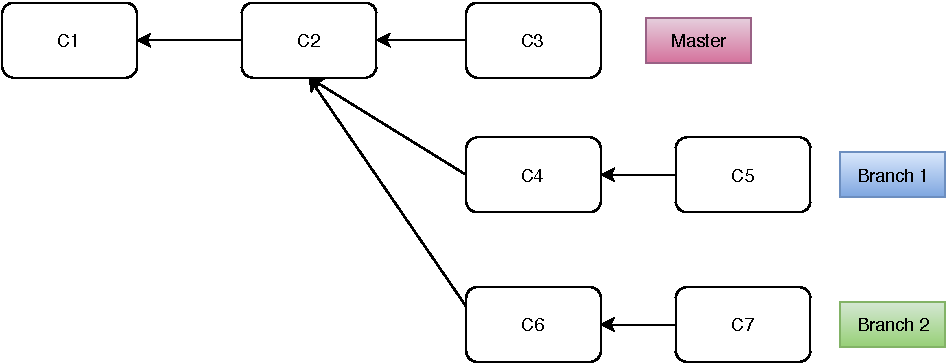
\includegraphics{capitulo_estudo_caso/exemplo_grafo_git.pdf} 
  \caption{Exemplo da estrutura de armazenamento de versões do Git.}
  \label{fig:cap_experimento_exemplo_grafo_git} 
\end{figure}

 \begin{figure}[H]
  \centering
  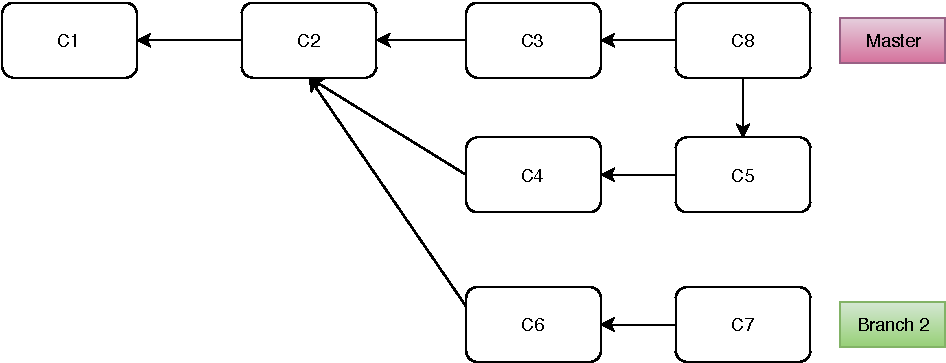
\includegraphics{capitulo_estudo_caso/exemplo_grafo_git_merge.pdf} 
  \caption{Exemplo de merge entre duas \textit{branches}.}
  \label{fig:cap_experimento_exemplo_grafo_git_merge} 
\end{figure}


\section{Comandos Git}
\label{ape:comandos_git}


A Tabela \ref{table:comandos_git} apresenta uma lista com os principais comandos do git.

\begin{table}[H]
\label{table:comandos_git}
\centering
\def\arraystretch{2.5}%
\begin{tabular}{|c|c|c|}
\hline
Comando & \pbox{6cm}{Descrição}                                                     & Exemplo                                     \\ \hline
clone   & \pbox{6cm}{Realiza uma cópia local de um repositório remoto }             & clone https://github.com/torvalds/linux.git \\ \hline
add     & \pbox{6cm}{Inclui um ou mais arquivos no gerenciamento de versão}         & add file.txt                                \\ \hline
commit  &\pbox{6cm} {Efetiva no histórico as mudanças realizadas}                   & commit -m ``History message"                 \\ \hline
push    & \pbox{6cm}{Envia as alterações locais para um repositório remoto}         & git push -u origin branch                   \\ \hline
pull    & \pbox{6cm}{Atualiza os arquivos locais com base em um repositório remoto} & git pull                                    \\ \hline
merge    & \pbox{6cm}{Realiza o merge entre duas \textit{branches}} & merge branch1                                 \\ \hline
branch    & \pbox{6cm}{Cria uma nova branch} & branch branch3                                 \\ \hline
checkout    & \pbox{6cm}{Muda o diretório de trabalho atual para uma determinada branch} & checkout branch3                                 \\ \hline
\end{tabular}
\caption{Comandos básicos do GIT.}
\label{table:comandos_git}
\end{table}

 
%\chapter{Banco de dados}
\label{apendice_banco_dados}      % associado ao arquivo: 'ape-conjuntos.tex'

% ---------------------------------------------------------------------------- %
% Bibliografia
\backmatter \singlespacing   % espaçamento simples
\bibliographystyle{alpha-ime}% citação bibliográfica alpha
\bibliography{bibliografia}  % associado ao arquivo: 'bibliografia.bib'

% ---------------------------------------------------------------------------- %
% Índice remissivo
%\index{TBP|see{periodicidade região codificante}}
%\index{DSP|see{processamento digital de sinais}}
%\index{STFT|see{transformada de Fourier de tempo reduzido}}
%\index{DFT|see{transformada discreta de Fourier}}
\index{Fourier!transformada|see{transformada de Fourier}}

\printindex   % imprime o índice remissivo no documento 

\end{document}
